% 1. Research summary (3 pages) describing the work in progress.
%    * 100-word abstract
%    * the expected contribution to the field of sensor networking
%    * the original idea or thesis statement
%    * the problem domain and the specific problem addressed
%    * a brief overview of related work
%    * the methodological approach
%    * research carried out and results so far.
% 2. Student biographical sketch, including the names and affiliations of the 
% research advisor, and expected date of dissertation submission. 

\documentclass[10pt]{sigplan-proc-varsize-sensys11}

\usepackage{fancyvrb}
\usepackage{booktabs}
\usepackage{colortbl}
\usepackage{tabularx}
\usepackage{multirow}
\usepackage{color}
\usepackage{xspace}
\usepackage{hyperref}    % Creates hyperlinks from ref/cite 
\hypersetup{pdfstartview=FitH}
\usepackage{graphicx}    % For importing graphics
\usepackage{url}         %

\renewcommand{\arraystretch}{1.2} % Space out rows in tables

\setlength\paperheight {11in}
\setlength\paperwidth {8.5in}

% No space between bibliography items:
\let\oldthebibliography=\thebibliography
  \let\endoldthebibliography=\endthebibliography
  \renewenvironment{thebibliography}[1]{%
    \begin{oldthebibliography}{#1}%
      \setlength{\parskip}{0ex}%
      \setlength{\itemsep}{0ex}%
  }%
  {%
    \end{oldthebibliography}%
  }
\setlength{\parindent}{5mm}

%%%%%%%%%%%%%%%%%%%%%%%%%%%%%%%%%%%%%%%%%%%%%%%%%%%%%%%%%%%%%%%%%%%%%%%%%%%%%%%

%\documentclass{sig-alternate}
%\documentclass{acm_proc_article-sp}

%\usepackage{fancyvrb}
\usepackage{verbatim}
\usepackage{amssymb}
\usepackage{amsmath}
\relpenalty=9999
\binoppenalty=9999

%\usepackage[pdftex]{graphicx}
%\usepackage{subfigure}

\newcommand{\2}{\;\;}
\newcommand{\5}{\;\;\;\;\;}
\newcommand{\til}{$\thicksim$}
\newcommand{\brk}{\textbf{\small{$^\wedge$}}}
\newcommand{\CEU}{\textsc{C\'{e}u}}
\newcommand{\code}[1] {{\small{\texttt{#1}}}}
\newcommand{\Code}[1] {\texttt{#1}}

\begin{document}

\title{C\'eu: A Reactive Language for Wireless Sensor Networks}

\author{
    {Francisco Sant'Anna} \\
    \affaddr{Departamento de Inform\'atica - PUC-Rio} \\
    \email{fsantanna@inf.puc-rio.br}
}

%\date{\today}

\conferenceinfo{SenSys'11,} {November 1--4, 2011, Seattle, WA, USA.}
\CopyrightYear{2011}
\crdata{XXX-X-XXXXX-XXX-X}

\maketitle

\begin{abstract}

\CEU{} is a system-level reactive language targeting Wireless Sensor Networks 
that poses an alternative to the predominating event-driven and threaded-based 
systems.
\CEU{} supports concurrent lines of execution that are allowed to share 
variables.
However, the static nature of \CEU{} enables a compile time analysis that 
ensures safe and deterministic execution.
The \CEU{} compiler generates single-threaded $C$ code that is comparable in 
size to handcrafted event-driven code.

\begin{comment}
For time consuming operations, \CEU{} provides asynchronous blocks that do not 
share state with the rest of the program.
As innovative features, \CEU{} introduces first-class support for 
\emph{physical time} (i.e. time from the real world), and simulation and 
testing from within the own programs.
\end{comment}

\end{abstract}

\section{Biography}
\label{sec.bio}

Francisco Sant'Anna is a second year Ph.D. student at PUC-Rio with expected 
graduation date in September, 2013.
His advisor is Roberto Ierusalimschy, associate professor at PUC-Rio in the 
field of programming languages, and the creator of the Lua language.
His co-advisor is Noemi de La Roque Rodriguez, associate professor at PUC-Rio 
in the field of distributed systems.

\section{Introduction}
\label{sec.intro}

Three aspects have been used to compare system programming languages for 
Wireless Sensor Networks: \emph{memory usage}, event processing 
(\emph{responsiveness}), and \emph{energy consumption} \cite{wsn.comparison}.

We consider that \emph{safety} is also an important aspect, as motes must run 
for long periods without human intervention.
In our discussion, we confine the term safety to deterministic and bounded 
execution (i.e.  programs should not execute long loops).
Current system languages for WSNs (e.g. \cite{wsn.tos, wsn.protothreads, 
wsn.mantisos}) do not detect such safety properties, requiring the programmer 
to perform exhaustive testing.
For instance, preemptive multithreading is non-deterministic by design, while 
event-driven and cooperative multithreading are susceptible to unbounded 
execution.

Finally, \emph{expressiveness} is another key aspect, regarding how programmers 
are able to write concise and maintainable programs.
Event-driven programming is intrinsically unstructured, while cooperative and 
preemptive mutilthreading require, respectively, explicit scheduling and 
synchronization, besides all exercise related to the life cycle of threads.

In our thesis, we present \CEU, a reactive language inspired in Esterel 
\cite{esterel.design} and FRP \cite{frp.fran} that aims to improve the safety 
and expressiveness of current system languages for WSNs.

\CEU{} relies on a compile-time analysis to detect unbounded loops and 
concurrent access to variables.
The static analysis forbids any dynamic support in the language, such as memory 
allocation, recursion, and dynamic loading.
However, this trade-off seems to be favorable in the context of WSNs, as 
dynamic features (such as \emph{malloc}) are discouraged due to the resource 
limitations and safety requirements.

WSNs applications typically react to multiple external events concurrently 
(e.g. timers, radio message arrivals, etc).
\CEU{} supports multiple lines of execution that can handle different events in 
parallel.
A line of execution can await an event without loosing context information, 
such as locals and the program counter.

\section{The Language C\'eu}
\label{sec.lang}

\CEU{} is a concurrent language in which multiple lines of execution (known as 
\emph{trails}) continuously react to input events from the environment.
Waiting for an event halts the running trail until that event occurs.
The environment broadcasts occurring events to all active trails, which share a 
single global time reference (an event itself).

The following example executes two trails in parallel that show in leds the 
received values from a radio:

%{\small
\begin{Verbatim}[commandchars=\\\{\}]
    (\til{}Radio_recv \til{}> v)* || (\til{}v \til{}> Leds_set)*
\end{Verbatim}
%}

The first trail (on the left of the \code{||} parallel operator) awaits 
(\code{\til}) the external input event $Radio\_recv$, then triggers 
(\code{\til>}) the internal event $v$, and then loops (\code{*}), repeating the 
process.
The second trail awaits the internal event $v$, then triggers the external 
output event $Leds\_set$, and then loops back.
In other words, whenever a radio message is received, the first trail resumes 
and awakes the second trail passing the received value through the internal 
event $v$.

The example could be simplified and rewritten just as
    \code{(\til{}Radio\_recv~\til{}>~Leds\_set)*},
but would not illustrate the concurrent nature of \CEU{}, though.

\newpage

The core BNF-like syntax of \CEU is the following:%
\footnote{We omitted the part of the language that borrows from $C$ type 
declarations, pointers, arrays, and constants from.}

\begin{figure}[ht]
\centering
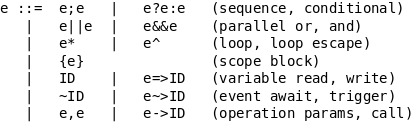
\includegraphics[scale=0.40]{figs/syntax.png}
\end{figure}

Note the syntax for attributions, triggers, and calls, where the source 
expressions come first (resembling a dataflow style).
Operators are defined conforming to a standard interface in a host language 
(e.g. functions in C).

A parallel expression executes its subexpressions in concurrent trails, 
terminating when one of them (\emph{par/or}), or both (\emph{par/and}) 
terminate.
All bookkeeping of trails (e.g. space allocation and scheduling) is done by the 
language, promoting a fine-grained use of trails.
For instance, when any expression in a \emph{par/or} terminates, \CEU{} 
automatically destroys all other sibling trails.

\begin{comment}
%{\small
\begin{verbatim}
  e ::= e;e    |  e?e:e   (sequence, conditional)
     |  e||e   |  e&&e    (parallel or, and)
     |  e*     |  e^      (loop, loop escape)
     |  {e}               (scope block)
     |  ID     |  e=>ID   (variable read, write)
     |  ~~ID   |  e~~>ID  (event await, trigger)
     |  e,e    |  e->ID   (operation params, call)
\end{verbatim}
%}

Follows the full syntax for \CEU{} expressions:
\emph{
    e;e        $|$    %(seq)
    e$||$e     $|$    %(paror)
    e\&\&e     $|$    %(parand) |
    e?e:e      $|$    %(cond)   |
    e*         $|$    %(loop)   |
    e\brk{}    $|$    %(break)  |
    a          $|$    %(load)   |
    e=$>$a     $|$
    \til{}a    $|$    %(await)  |
    e\til$>$a  $|$
    e--$>$op   $|$
    e,e        $|$    %(parand) |
    K},
corresponding respectively to sequence, parallel/or, parallel/and, conditional, 
loop, loop break, variable read/write, event await/trigger, operation 
params/call, and constant value.
Parallel constructs execute their subexpressions concurrently, terminating when 
one of its subexpressions terminate (\emph{par/or}) or both (\emph{par/and}).
Operators are defined externally, conforming to a standard interface in a host 
language (e.g. functions in C).
\end{comment}

\CEU{} is grounded on a precise definition of time as \emph{a discrete sequence 
of external input events}: a sequence because only a single input event is 
handled at a time; discrete because a complete reaction always executes in 
bounded time (discussed in Section~\ref{sec.safety}).
The execution model for a \CEU{} program is as follows:

\begin{enumerate}
\item The program initiates in a single trail.
\item Active trails execute until they await or terminate.
      This step is named as a \emph{reaction chain}, and always runs in bounded 
      time.
\item If the program does not terminate, then it goes idle and the environment 
      takes the control.
\item On the occurrence of a new input event, the environment awakes the 
      program on its awaiting trails.
      Then, goes to step 2.
\end{enumerate}

If a new input event happens while a reaction chain (step 2) is running, the 
environment enqueues it, as reaction chains must run to completion.
When multiple trails are active at a time, \CEU{} does not specify the order in 
which they should execute.
The language runtime is allowed to serialize, interleave, or even parallelize 
their execution.

Every variable in \CEU{} is also an internal event and vice-versa.
By triggering an internal event with a value also assigns that value to it.
For this reason, internal events are also known as \emph{reactive variables}.
The following program fragment specifies that whenever the variable $v1$ 
changes, $v2$ is automatically updated to the increment of $v1$, which in turn, 
automatically updates $v3$ to the increment of $v2$:

\Code{(\til{}v1->inc \til{}> v2)* || (\til{}v2->inc \til{}> v3)*}

In contrast with external events, which are handled in a queue, internal events 
follow a stack policy and react within the same propagation chain.
In practical terms, this means that a trail that triggers an internal event 
halts until all trails awaiting that event completely react to it, continuing 
to execute afterwards, but within the same time unit.

\section{Safety}
\label{sec.safety}

A reaction chain must run in bounded time to ensure that a program is 
responsive and can handle upcoming events.
In \CEU, only \emph{operators} and \emph{loops} might cause a reaction chain to 
run in unbounded time.

As operators are typically simple functions that provide ordinary operations, 
\CEU{} assumes that their implementation in the host language do not enter in 
loop.

For \CEU{} \emph{loops}, we restrict that they must contain at least one 
\emph{await} or \emph{break} expression on theirs bodies for each possible path 
within them.
For instance, based on this restriction, the following loops are refused at 
compile time:
\code{(1)*}, \code{(\til{}A||v)*}, \code{(v?1:\til{}A)*}; while the following 
are accepted: \code{(\til{}A)*}, \code{(\til{}A\&\&v)*}, \code{(\til{}A?1:0)*}.
By structural induction, it is trivial to infer whether a given loop body 
expression holds this restriction or not.

% TODO: claim desired property
Determinism is usually a desired safety property, making programs 
more predictable and easier to debug.
% TODO: prove
In \CEU, there are three possible sources of non-determinism:
\emph{concurrent access to variables} (e.g. \code{(1=>a\&\&2=>a)}),
\emph{concurrent \emph{par/or} termination} (e.g. \code{(1||2)=>a}, might yield 
$1$ or $2$), and \emph{concurrent loop escape}%
\footnote{ The token \brk{} escapes the innermost loop with its preceding 
expression. }
(e.g. \code{(1\brk{} \&\& 2\brk)* =>a}).

During compile time, \CEU{} converts programs into deterministic finite 
automatons in order to detect the three forms of non-determinism.
This conversion is the reason why \CEU{} is a static language.
% TODO: claim
A DFA unequivocally represents a \CEU{} program, covering exactly all possible 
paths it can reach during runtime.
For instance, the following program is identified as non-deterministic, because 
the variable $v$ is accessed concurrently on the 6th occurrence of the event 
$A$:

\Code{
(\til{}A; \til{}A; 1=>v)*
\&\&
(\til{}A; \til{}A; \til{}A; v)*
}

\begin{comment}
Figure~\ref{fig.dfa_02} shows the resulting DFA for the program%
\footnote{
    The subscripts help identifying each \code{\til{}A}, but are not part of 
the program.
}

Each state contains what to execute and what to await.
For instance, the first state represents both trails awaiting the event $A$.
After six occurrences of $A$, the variable $v$ is accessed concurrently in both 
trails (in the dotted state), qualifying a non-deterministic behavior in the 
program, which is refused at compile time.

\begin{figure}[ht]
\centering
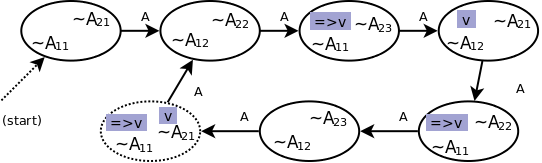
\includegraphics[scale=0.30]{figs/dfa_02.png}
\caption{ DFA for a non-deterministic program. }
\label{fig.dfa_02}
\end{figure}

%TODO: pointers \& arrays
\end{comment}

\section{Physical Time}
\label{sec.time}

% TODO: claim most commonly used
\emph{Physical time}%
\footnote{
By physical time we mean the passage of time from the real world, measured in 
hours, minutes, milliseconds, etc.
}
is probably the most common input in WSN applications, as found in typical 
patterns, such as sensor sampling, and watchdogs.
However, system languages support for physical time is somewhat low-level, 
usually through \emph{timer} callbacks or \emph{sleep} blocking calls.
\CEU{} provides a first-class support for physical time: the expression 
\code{\til{}1s500ms} awaits one second and a half.

\CEU{} takes into account the fact that time is a physical quantity that can be 
added and compared.
For instance, in the expression \code{(\til{}50ms;\til{}49ms~||~\til{}100ms)}, 
if \CEU{} cannot guarantee that the left \emph{par/or} subexpression terminates 
exactly in 99ms, it can at least ensure that it will terminate before the 
second subexpression does.
Likewise, in the expression \code{(\til{}10ms)*}, after 1 second elapses, the 
loop iterated exactly 100 times, even if a given reaction chain during that 
period takes longer than $20ms$.

Finally, the temporal analysis of \CEU{} (shown in previous section) also 
embraces the semantics for time.
The expression \code{(\til{}50ms;\til{}49ms;1=>a~||~\til{}100ms;2=>a)}
is deterministic, while \code{((\til{}10ms;1=>a)*~||~\til{}100ms;2=>a)} is not.

\section{Evaluation}
\label{sec.evaluation}

\newcommand{\fr}{{\small$^{\CEU}/_{nesC}$}}
\newcommand{\s}[1]{{\small \textbf{#1}}}

From the aspects we want to evaluate in \CEU ---\emph{memory} and 
\emph{battery} consumption, \emph{responsiveness}, \emph{safety}, and 
\emph{expressiveness}--- we already have quantitative measures for memory usage 
and expressiveness (in terms of source code size).

We ported existing TinyOS/nesC%
\footnote {
    We chose to use TinyOS due to its simplicity and acceptance in the WSN 
    community.
    We are using $TinyOS-2.1.1$ and $micaz$ motes in our experiments.
}%
\cite{wsn.tos} applications to \CEU{} to support our experiments.
The following table shows the measures for ROM, RAM, and LOCs (lines of code) 
for the same applications written in nesC and \CEU{}.
The third line for each application shows the ratio \fr{} for a given measure, 
for example: the AntiTheft written in \CEU{} uses $1.40$ times more RAM than 
its nesC counterpart.

\begin{table}[h]\small
%\caption{Comparison of system-level languages models for WSNs.}
\label{tab.evaluation}
\begin{center}
\begin{tabular}{ | l | r | r | r | r | }
\hline
\multicolumn{2}{|c|}{}
           &         ROM &         RAM &       LOC \\
\hline\hline

\multirow{3}{*}{Blink}
    & nesC &  2052 bytes &    51 bytes &  17 lines \\
    & \CEU &  4168 bytes &   247 bytes &   5 lines \\
    &  \fr &    \s{2.03} &    \s{4.84} &  \s{0.29} \\
\hline\hline

\multirow{3}{*}{Sense}
    & nesC &  4370 bytes &    84 bytes &  24 lines \\
    & \CEU &  6742 bytes &   348 bytes &  11 lines \\
    &  \fr &  \s{1.54}   &    \s{4.14} &  \s{0.46} \\
\hline\hline

\multirow{3}{*}{AntiTheft}
    & nesC & 22424 bytes &  1663 bytes &  85 lines \\
    & \CEU & 27014 bytes &  2325 bytes &  45 lines \\
    &  \fr &    \s{1.20} &    \s{1.40} &  \s{0.53} \\
\hline\hline

\multirow{3}{*}{BaseStation}
    & nesC & 15216 bytes &  1735 bytes & 144 lines \\
    & \CEU & 19844 bytes &  2373 bytes &  57 lines \\
    &  \fr &    \s{1.30} &    \s{1.37} &  \s{0.40} \\
\hline

\end{tabular}
\end{center}
\end{table}

Our experiments suggest that as the applications complexity grows, the 
difference in memory consumption decreases, reaching around 30-35\% for the 
BaseStation application.
This behavior is a consequence of the memory footprint of \CEU{}, which 
requires specialized code for the runtime bookkeeping of timers, trails, 
events, etc.

When evaluating LOCs of programs, we considered only their core implementation
file (\emph{modules} in nesC), and extracted from it all comments, interface 
declarations, and extra spaces.%
\footnote{
    The original and modified sources for the experiments can be found at
    {\small\url{www.lua.inf.puc-rio.br/~francisco/sensys\_11.html}}.
}
With this approach we focused on the logic of programs, where programmers spend 
most of their time and rely on the expressiveness of the language in use.
The \CEU{} numbers are quite satisfactory, being around $50\%$ smaller for all 
applications.

\section{Related Work}

Our work is influenced by the Esterel language \cite{esterel.design}, an 
imperative reactive language with similar constructs.
Karpinski and Cahill \cite{wsn.sol} present a language targeting WSNs (also 
based on Esterel), and perform a throughout quantitative and qualitative 
comparison with nesC.
\CEU{} differs from these languages with its semantics for internal events, 
physical time, and a more consistent support for concurrent access to 
variables.
 
Protothreads \cite{wsn.protothreads} offer very lightweight threads with 
blocking support.
Its stackless implementation reduces memory consumption but prevents automatic 
variables.
Protothreads provide no safety support besides atomic execution of threads:
a program can loop indefinitely, and access to globals is unrestricted.

\section{Conclusion}
\label{sec.conclusion}

We believe that \CEU{} poses concrete advantages in terms of safety and 
expressiveness when compared to current system languages for WSNs.
Regarding safety, we propose a temporal analysis of programs that prevents 
unresponsiveness and enforces deterministic behavior.
In terms of expressiveness, our initial experiments show a 50\% decrease in 
LOCs when comparing \CEU{} to nesC.

In the design of \CEU{} we favored safety over power, since we restricted the 
language to static capabilities only.
However, this limitation can be considered (to some extent) advantageous for 
WSNs, given that \CEU{} enforces the prevailing discipline in this context.

At this point, we did not evaluate battery consumption and responsiveness 
aspects, but we plan to perform quantitative analysis for them.
Responsiveness, in particular, deals with long running tasks that currently 
require explicit yields inside loops (e.g. with \code{\til{}1ms}).
We are working on a lightweight asynchronous extension to \CEU{} to address 
this limitation.

\begin{comment}
On the implementation size, \CEU{} currently uses redundant registers that 
increase memory consumption considerably.
Hence, it is possible to achieve better results in this aspect.
\end{comment}

We intend to port more complex applications to \CEU{} to improve our 
evaluation.
We are aware of the limitations of evaluating the expressiveness of \CEU{} 
based solely on LOCs, though.
On the way to a more in-depth qualitative approach, we are teaching \CEU{} as 
an alternative to nesC in introductory courses on WSNs for undergraduate and 
also high school students.
We will compare the achievements of the students with both models and use the 
results in our evaluation.

\begin{comment}

With a similar approach,
SOL, heavy syntax, what about additional space(stack)
comparacao como artigo HIGH
incluir linhas de codigo

Finally, SOL \cite{} is a Esterel-like language targeting WSNs.
Also, Table~\ref{} and we show equivalent results for ROM and RAM.

Similar evaluation in a previous work \cite{wsn.sol}.

Safety
Expressivenes: physical time

precisamos de mais exemplos

coarse grained vs fine grained multithreading

auto book allows fine-graining

ceu is stackless

also syntactic support

falar de composibility

bateria, uso de memoria igual, a nao ser que o programa perca tempo em coisas 
que os outros nao fazem
em relacao a threads, no context switch
mesmo para os asyncs nao ha context switch
no run-time overheads due to threads creation/destroy, just set flags

nondet for Pars/raises

% TODO: claim recurrent use justifies
We believe that the recurrent use of physical time in reactive applications 
already justifies providing a convenient syntax for timing purposes.
Furthermore, native support is also \emph{desired} to avoid dealing explicitly 
with \emph{residual delta times} from expired timers; and is \emph{required} to 
allow extending \CEU's temporal analysis to include physical time.

\end{comment}

{\footnotesize
\bibliographystyle{abbrv}
\bibliography{other}
}

\begin{comment}
\begin{table}[h]\small
%\caption{Comparison of system-level languages models for WSNs.}
\label{tab.evaluation}
\begin{center}
\begin{tabular}{ | l | r | r | r | r | }
\hline
\multicolumn{2}{|c|}{}
           & ROM (bytes) & RAM (bytes) & LOC (lines) \\
\hline\hline

\multirow{3}{*}{Simplest}
    & nesC &        616  &          4  &          1  \\
    & \CEU &       3792  &        195  &          1  \\
    &  \fr &    \s{6.16} &   \s{48.75} &    \s{1.00} \\
\hline\hline

\multirow{3}{*}{Blink}
    & nesC &       2052  &         51  &         17  \\
    & \CEU &       4316  &        203  &          5  \\
    &  \fr &    \s{2.10} &    \s{3.98} &    \s{0.29} \\
\hline\hline

\multirow{3}{*}{Sense}
    & nesC &     4370    &         84  &         24  \\
    & \CEU &     7084    &        354  &         11  \\
    &  \fr &  \s{1.62}   &    \s{4.21} &    \s{0.46} \\
\hline\hline

\multirow{3}{*}{BaseStation}
    & nesC &      15216  &       1735  &        145  \\
    & \CEU &      21352  &       2394  &         65  \\
    &  \fr &    \s{1.40} &    \s{1.38} &    \s{0.45} \\
\hline\hline

\multirow{3}{*}{AntiTheft}
    & nesC &      00000  &       0000  &        000  \\
    & \CEU &      00000  &       0000  &        000  \\
    &  \fr &    \s{1.00} &    \s{1.00} &    \s{0.00} \\
\hline

\end{tabular}
\end{center}
\end{table}

\begin{table}[h]\small
%\caption{Comparison of system-level languages models for WSNs.}
\label{tab.evaluation}
\begin{center}
\begin{tabular}{ | l | c | c | c | c | }
\hline
\multicolumn{2}{|c|}{}
           & ROM (bytes) & RAM (bytes) & LOC (lines) \\
\hline\hline

\multirow{3}{*}{Simplest}
    & nesC &        616  &          4  &          1  \\
    & \CEU &       3792  &        195  &          1  \\
    &  \fr &    \s{6.16} &   \s{48.75} &    \s{1.00} \\
\hline\hline

\multirow{3}{*}{Blink}
    & nesC &       2052  &         51  &         17  \\
    & \CEU &       4316  &        203  &          5  \\
    &  \fr &    \s{2.10} &    \s{3.98} &    \s{0.29} \\
\hline\hline

\multirow{3}{*}{Sense}
    & nesC &     4370    &         84  &         24  \\
    & \CEU &     7084    &        354  &         11  \\
    &  \fr &  \s{1.62}   &    \s{4.21} &    \s{0.46} \\
\hline\hline

\multirow{3}{*}{BaseStation}
    & nesC &      15216  &       1735  &        145  \\
    & \CEU &      21352  &       2394  &         65  \\
    &  \fr &    \s{1.40} &    \s{1.38} &    \s{0.45} \\
\hline\hline

\multirow{3}{*}{AntiTheft}
    & nesC &      00000  &       0000  &        000  \\
    & \CEU &      00000  &       0000  &        000  \\
    &  \fr &    \s{1.00} &    \s{1.00} &    \s{0.00} \\
\hline

\end{tabular}
\end{center}
\end{table}
\end{comment}

\end{document}
